
%(BEGIN_QUESTION)
% Copyright 2015, Tony R. Kuphaldt, released under the Creative Commons Attribution License (v 1.0)
% This means you may do almost anything with this work of mine, so long as you give me proper credit

Analyze the status of all relay contacts and lamps in this hard-wired relay ``ladder logic'' control circuit:

$$\includegraphics[width=15.5cm]{i02605x01.eps}$$

Assume the following input conditions:

\begin{itemize}
\item{} Pushbutton switch {\it unpressed}
\item{} Pressure {\it above} trip threshold
\item{} Selector switch in its {\it right-hand} position
\end{itemize}

\vfil \eject

Now, analyze the status of this PLC-controlled system assuming the same input conditions.  Note the distinction between the 120 VAC circuitry and the ``virtual circuit'' in the blue-shaded area representing the program executed by the PLC's microprocessor:

$$\includegraphics[width=15.5cm]{i02605x02.eps}$$

\begin{itemize}
\item{} Pushbutton switch {\it unpressed}
\item{} Pressure {\it above} trip threshold
\item{} Selector switch in its {\it right-hand} position
\end{itemize}

How is the PLC-controlled system similar to the hard-wired relay control system?  How is it different?

\vskip 10pt

\underbar{file i02605}
%(END_QUESTION)





%(BEGIN_ANSWER)

A good problem-solving technique to apply in both diagrams is {\it annotation}, where you indicate the presence of continuity and power versus non-continuity/unpowered.  In PLC programs this usually appears in the form of color-highlighting surrounding each instruction symbol (virtual contact or virtual coil).

%(END_ANSWER)





%(BEGIN_NOTES)

Analysis of hard-wired relay control circuit:

$$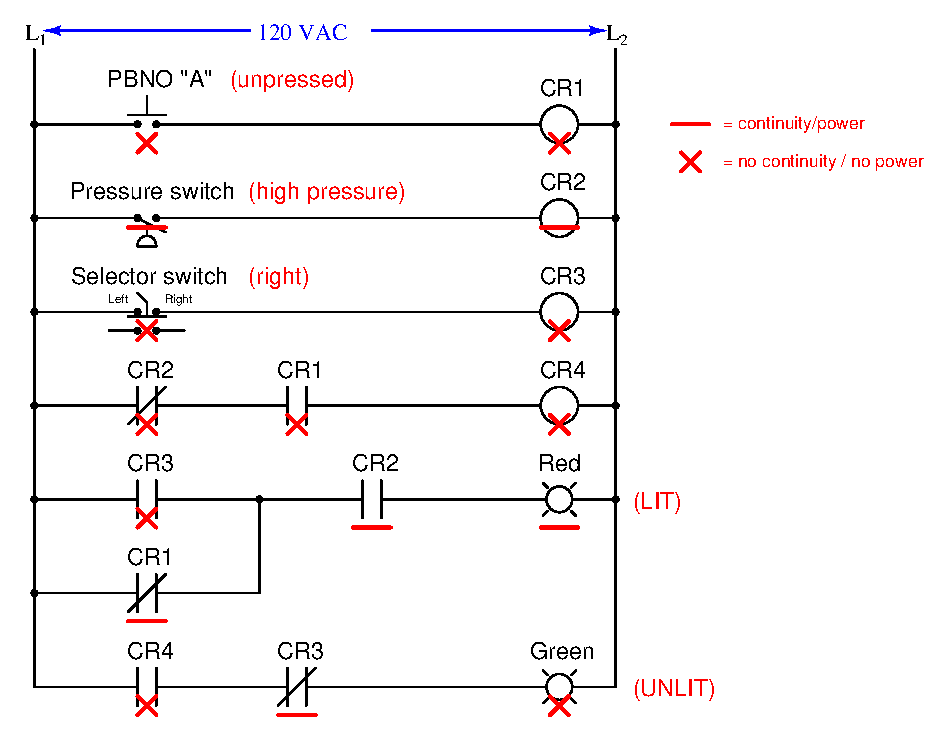
\includegraphics[width=15.5cm]{i02605x03.eps}$$

\vfil \eject

Analysis of PLC-controlled circuit:

$$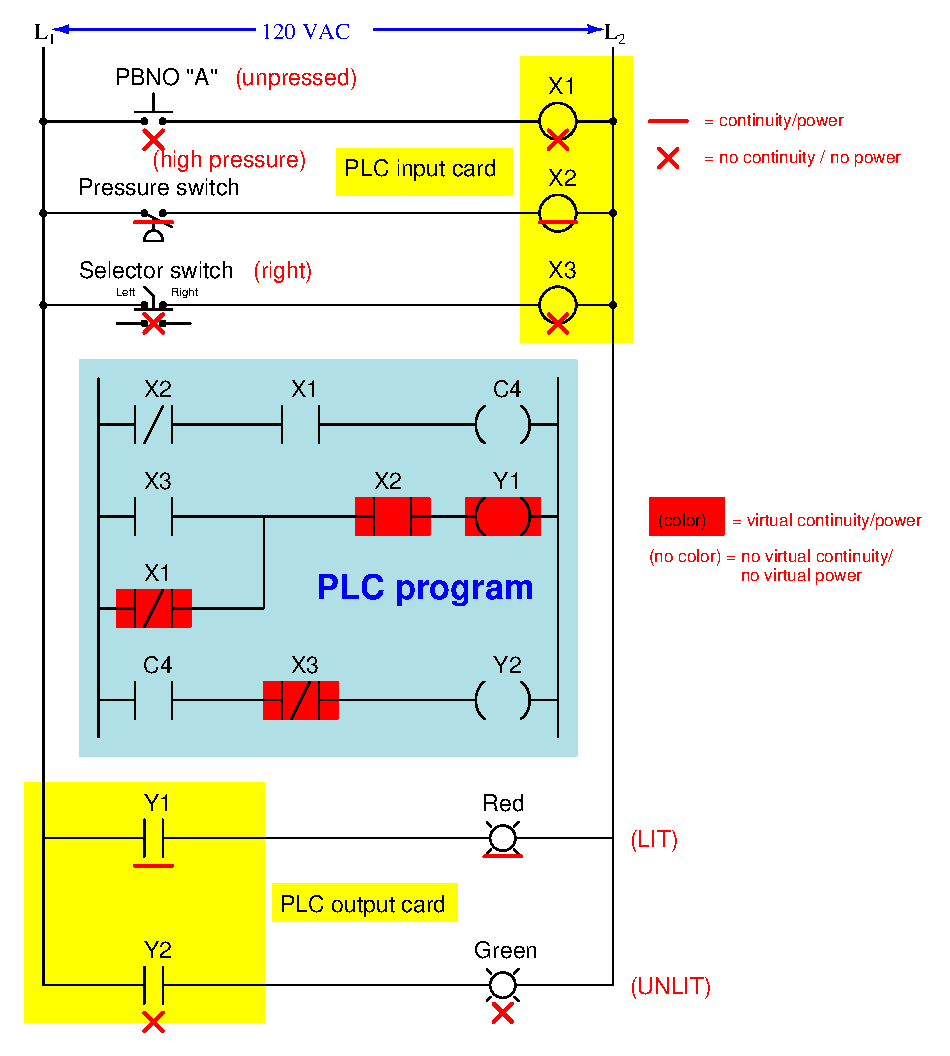
\includegraphics[width=15.5cm]{i02605x04.eps}$$

%INDEX% PLC, relating I/O status to virtual elements (analogy to relay ladder logic circuitry)

%(END_NOTES)


